\chapter{声学拓扑晶体绝缘体的理论建模}
\section{引言}

\section{电声类比方法}

由于我们在用声学实现拓扑效应时,很多情况下是利用腔管共振结构实现声学结构和电子晶格结构的对应。而在声学研究中,电声类比是研究这类结构的一种常用方法。它适用于结构尺寸远小于波长的情况,是一种将集总参数的电路系统和声学系统进行类比分析的有效手段。它基于电学和声学在某些物理特性和数学描述上的相似性,建立起两者之间的对应关系,从而借助电学中成熟的理论和分析方法来研究声学问题。
在这种类比中,电学中的电压、电流、电阻、电容、电感等概念分别与声学中的声压、体积速度、声阻、声容、声感等概念相对应。通过电声类比,我们可以将复杂的声学系统转化为等效的电学电路模型,利用电路分析的方法来求解声学系统的特性,因此本节首先介绍这种方法。

\subsection{声容}

\begin{figure}[h!]
  \centering
  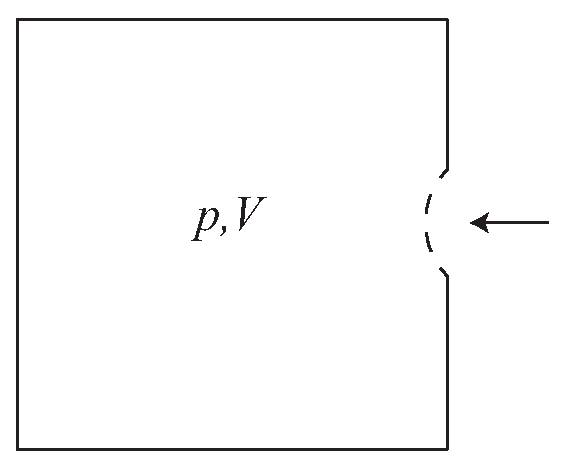
\includegraphics[width=0.5\textwidth]{images/fig2-1.eps} 
  \caption{声容示意图 }
  \label{fig_2_1}
\end{figure}

对于一个壁面为刚性边界且带开口的腔体,当腔体里面的空气振动时,其声压和体积变化存在着某种关系。当开口较小且波长远大于结构尺寸时,这种关系往往是线性化的。我们可以把这样的结构称为声容,如图\ref{fig_2_1}。声容的推导从绝热近似的状态方程出发,假设声波传播过程为绝热过程,则
\begin{equation} \label{eq2-1}
  pV^\gamma = \text{常数},
\end{equation}
其中 \(p\) 为气体压力,\(V\) 为气体体积,\(\gamma = \frac{C_p}{C_v}\) 为绝热指数。对该公式取对数后对时间求导,得到
\begin{equation} \label{eq2-2}
  V^\gamma \frac{dp}{dt} + \gamma p V^{\gamma-1} \frac{dV}{dt} = 0,
\end{equation}
整理为
\begin{equation} \label{eq2-3}
  \frac{dp}{p} + \gamma \frac{dV}{V} = 0,
\end{equation}
假设声波的压力和体积变化为微小量,即
\begin{equation} \label{eq2-4}
  p = p_0 + \Delta p, \quad V = V_0 + \Delta V,
\end{equation}
代入后忽略高阶小量项,得
\begin{equation} \label{eq2-5}
  \frac{\Delta p}{p_0} = -\gamma \frac{\Delta V}{V_0},
\end{equation}
从中可得体积变化和压力变化之间的关系为
\begin{equation} \label{eq2-6}
  \Delta V = -\frac{V_0}{\gamma p_0} \Delta p
\end{equation}
声容 \(C_a\) 定义为单位压力变化引起的体积变化:
\begin{equation} \label{eq2-7}
  C_a = \frac{\Delta V}{\Delta p},
\end{equation}
将上述关系式代入后得到
\begin{equation} \label{eq2-8}
  C_a = \frac{V_0}{\gamma p_0},
\end{equation}
进一步结合声速的定义
\begin{equation} \label{eq2-9}
  c^2 = \frac{\gamma p_0}{\rho_0},
\end{equation}
将 \(\gamma p_0\) 替换为 \(\rho_0 c^2\),最终得声容的表达式
\begin{equation} \label{eq2-10}
  C_a = \frac{V}{\rho_0 c^2},
\end{equation}
这一公式揭示了声容取决于腔体体积 \(V\)、介质密度 \(\rho_0\) 和声速 \(c\),其中声容越大表示腔体对压力变化的响应越显著。

\subsection{声质量}

\begin{figure}[h!]
  \centering
  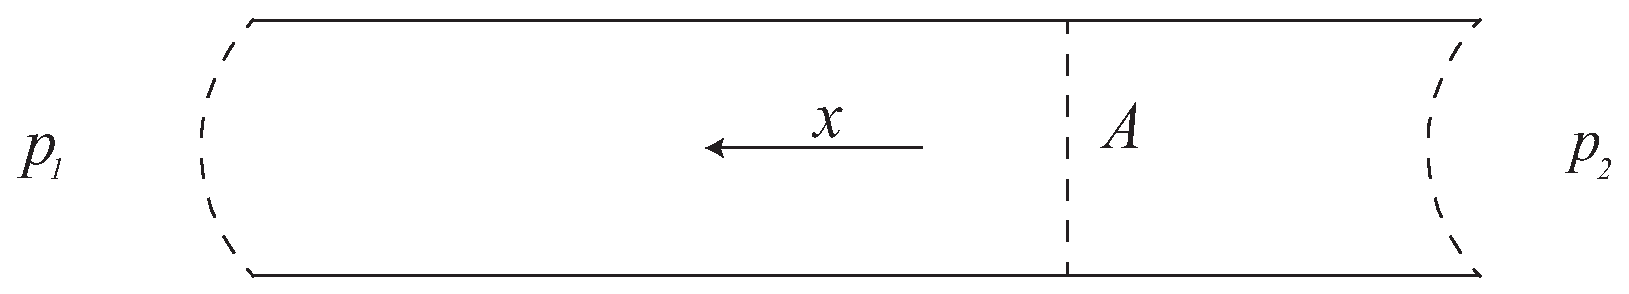
\includegraphics[width=0.5\textwidth]{images/fig2-2.eps} 
  \caption{声质量示意图 }
  \label{fig_2_2}
\end{figure}

当短管足够小,我们可以认为短管里的空气是整体振动的,此时可以把它视作质点,或者声质量,如图\ref{fig_2_2}。声质量的推导从牛顿第二定律开始。假设在声学系统中,颈管内的空气柱被视为振动的质点,其运动遵循牛顿第二定律:
\begin{equation} \label{eq2-11}
  F = M \frac{d^2 x}{dt^2},
\end{equation}
其中 \( F \) 为作用在空气柱上的力,\( M \) 为空气柱的质量,\( x \) 为空气柱的位移。对于声波传播,作用力由声压差产生,可以表示为:
\begin{equation} \label{eq2-12}
  F = \Delta p \cdot A,
\end{equation}
其中 \( \Delta p \) 为两端声压差,\( A \) 为颈管的截面积。空气柱的质量 \( M \) 表示为:
\begin{equation} \label{eq2-13}
  M = \rho_0 l_{\text{eff}} A,
\end{equation}
其中 \( \rho_0 \) 为空气的静态密度,\( l_{\text{eff}} \) 为颈管的有效长度,考虑了端点修正(通常为 \( l + 1.7r \),其中 \( r \) 是颈管半径)。将 \( F \) 和 \( M \) 表达式代入牛顿第二定律,得到:
\begin{equation} \label{eq2-14}
  \Delta p \cdot A = \rho_0 l_{\text{eff}} A \frac{d^2 x}{dt^2},
\end{equation}
简化为:
\begin{equation} \label{eq2-15}
  \Delta p = \rho_0 l_{\text{eff}} \frac{d^2 x}{dt^2},
\end{equation}
由体积流量 \( U \) 的定义,\( U = A \frac{dx}{dt} \),两次对时间求导后,得到空气柱的加速度与体积流量的关系:
\begin{equation} \label{eq2-16}
  \frac{d^2 x}{dt^2} = \frac{1}{A} \frac{dU}{dt},
\end{equation}
代入上述公式,得到:
\begin{equation} \label{eq2-17}
  \Delta p = \rho_0 l_{\text{eff}} \frac{1}{A} \frac{dU}{dt},
\end{equation}
整理后可得空气柱的声质量表达式:
\begin{equation} \label{eq2-18}
  L_a = \frac{\rho_0 l_{\text{eff}}}{A},
\end{equation}
这一公式表明,声质量 \( L_a \) 是由空气的静态密度 \(\rho_0\)、颈管的有效长度 \(l_{\text{eff}}\) 和截面积 \(A\) 决定的,其中 \( L_a \) 越大,表示空气柱对流量变化的惯性越强。

\subsection{声阻}
短管中的空气振动时,往往会收到壁面的阻力,线性化且集总参数的情况下,阻力的大小被视为和速度成正比。声阻的推导从牛顿第二定律和流体动力学的基本方程出发,描述了声波传播时介质中摩擦力引起的阻力。假设声波通过一个窄管时,声阻力来源于空气柱在运动过程中与管壁之间的黏性摩擦。牛顿第二定律为:
\begin{equation} \label{eq2-19}
  F = M \frac{d^2 x}{dt^2},
\end{equation}
其中 \( F \) 是作用在空气柱上的总力,\( M \) 是空气柱的质量,\( x \) 是空气柱的位移。在考虑摩擦力的情况下,总力 \( F \) 包含两个分量:由压力差引起的驱动力 \( F_p = \Delta p \cdot A \) 和与速度成正比的阻力 \( F_r = R_a \frac{dx}{dt} \),其中 \( R_a \) 是声阻。由此,总力可以表示为:
\begin{equation} \label{eq2-20}
  \Delta p \cdot A - R_a \frac{dx}{dt} = M \frac{d^2 x}{dt^2},
\end{equation}
空气柱的质量 \( M \) 表达为:
\begin{equation} \label{eq2-21}
  M = \rho_0 l A,
\end{equation}
其中 \( \rho_0 \) 为空气密度,\( l \) 为空气柱的长度,\( A \) 为管道的截面积。将体积流量 \( U = A \frac{dx}{dt} \) 代入,声压差与流量的关系变为:
\begin{equation} \label{eq2-22}
  \Delta p = R_a \frac{U}{A} + \rho_0 l \frac{1}{A} \frac{dU}{dt},
\end{equation}
忽略惯性项(即空气柱的质量效应较小的情况下),可以得到声阻的定义:
\begin{equation} \label{eq2-23}
  R_a = \frac{\Delta p}{\frac{U}{A}},
\end{equation}
对于圆形管道,声阻可以进一步结合流体动力学中的黏性摩擦公式推导,其值为:
\begin{equation} \label{eq2-24}
  R_a = \frac{8 \mu l}{\pi r^4},
\end{equation}
其中 \( \mu \) 是空气的动态黏性系数,\( l \) 是管道的长度,\( r \) 是管道的半径。这一公式表明,声阻 \( R_a \) 与介质的黏性和管道的几何尺寸(长度和半径)直接相关,管道越窄,声阻越大,黏性越强,声阻也越大,从而对体积流量的变化产生显著的阻碍作用。





